%
%  Wakefield Acceleration
% ========================
%

\chapter{A Wakefield Accelerator Experiment}
\label{Ch:WFA}

\begin{figure}[hbt]
    \centering
    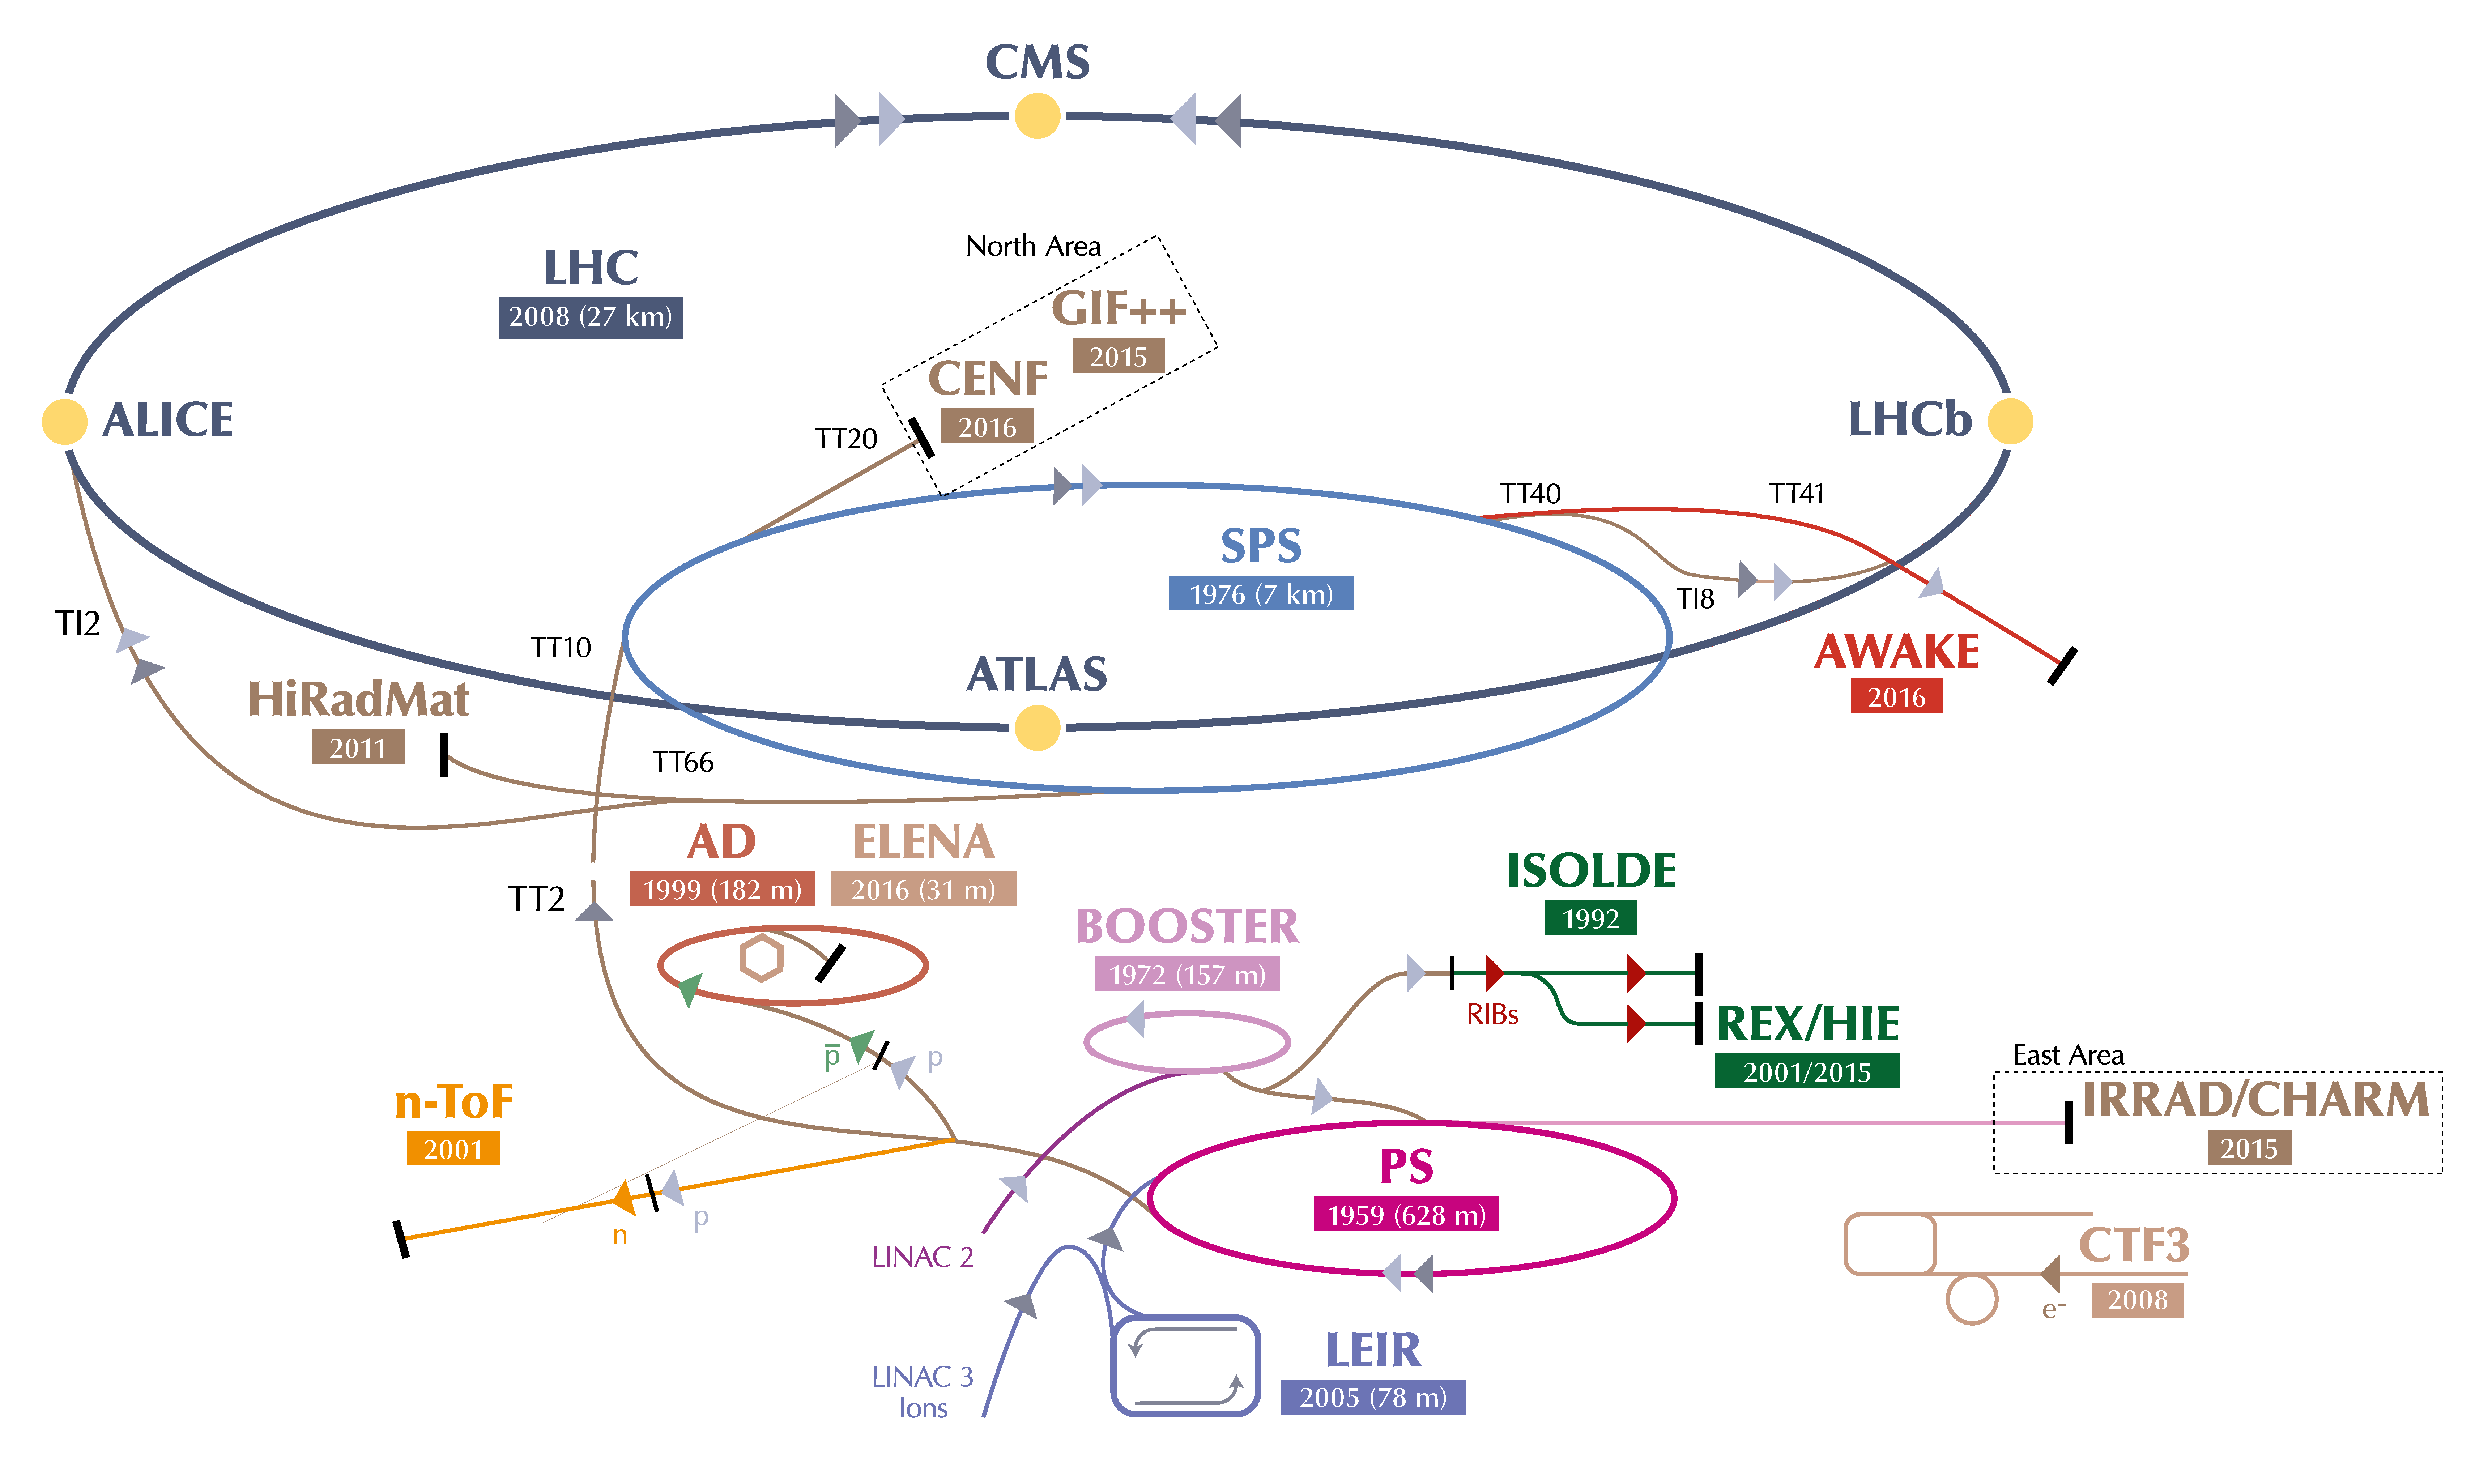
\includegraphics[width=0.99\linewidth,trim={20mm 25mm 20mm 20mm},clip]{figures/AcceleratorComplex}
    \caption{\label{Fig:WFA:AccComp}
        An overview of the CERN Accelerator Complex \cite{add:mobs:2016}.}
\end{figure}

Introduction

Intro paper \cite{caldwell:2009}

Launch paper \cite{awake_collaboration:2014}

Evolution paper \cite{caldwell:2016}

Technical specs \cite{gschwendtner:2016}

Status report \cite{awake_collaboration:2016}

% ================================================================================================ %
\section{Evolution of the Concept}
\label{WFA:History}

Previous experiments, SLAC, etc.

\cite{rosenzweig:1988, blumenfeld:2007, kallos:2008, litos:2014}

Self modulation at FACET \cite{adli:2016}

Review by Patric \cite{muggli:2009}

% ================================================================================================ %
\section{The Advanced Wakefield Experiment (AWAKE)}
\label{WFA:AWAKE}

A summary of the AWAKE experiment

% ================================================================================================ %
\subsection{AWAKE Run 1}
\label{WFA:AWAKE:R1}

Description of Run 1. SMI, long e-beam.

% ================================================================================================ %
\subsection{AWAKE Run 2}
\label{WFA:AWAKE:R2}

Short e-beam, multiple stages, etc.

Problems relevant for this thesis.

Erik \cite{adli:2016a}

% ================================================================================================ %
\section{The Self-modulation Instability in AWAKE}
\label{WFA:SMI}

Results from Run 1 of the experiment.

% ================================================================================================ %
